\documentclass[10pt]{article}
\usepackage{hyperref}
\usepackage[T1]{fontenc}
\usepackage[latin1]{inputenc}
%\usepackage{beton}
%\usepackage{ccfonts}
%\usepackage{concrete}
\usepackage{concmath}
\usepackage{eulervm}
\usepackage{amsmath,amsthm,amssymb}
\usepackage{mathtools}
\usepackage{multicol}
\usepackage{marginnote}
\usepackage{pgfplots}
\usepackage{float}
\usepackage{hyperref}
\pgfplotsset{compat=1.5}
\usepackage{graphicx}
\graphicspath{ {./images/} }
\usepackage{listings}
\usepackage{xcolor}
\definecolor{codegreen}{rgb}{0,0.6,0}
\definecolor{codegray}{rgb}{0.5,0.5,0.5}
\definecolor{codepurple}{rgb}{0.58,0,0.82}
\definecolor{backcolour}{rgb}{0.95,0.95,0.92}
\lstdefinestyle{mystyle}{
    backgroundcolor=\color{backcolour},   
    commentstyle=\color{codegreen},
    keywordstyle=\color{magenta},
    numberstyle=\tiny\color{codegray},
    stringstyle=\color{codepurple},
    basicstyle=\ttfamily\footnotesize,
    breakatwhitespace=false,         
    breaklines=true,                 
    captionpos=b,                    
    keepspaces=true,                 
    numbers=left,                    
    numbersep=5pt,                  
    showspaces=false,                
    showstringspaces=false,
    showtabs=false,                  
    tabsize=2
}

\lstset{style=mystyle}

\usepackage{mathtools}

\usepackage{wasysym}
\usepackage[margin=1.5in]{geometry} 
\usepackage{enumerate}
\index{\usepackage}\usepackage{multicol}

\newcommand{\N}{\mathbf{N}}
\newcommand{\Z}{\mathbb{Z}}

\newcommand{\R}{\mathbf{R}}
\newcommand{\C}{\mathbf{C}}
\newcommand{\Pbb}{\mathbb{P}}
\newcommand{\Fcal}{\mathcal{F}}
\newcommand{\Acal}{\mathcal{A}}
\newcommand{\Ecal}{\mathcal{E}}
\newcommand{\Ebb}{\mathbb{E}}
\newcommand{\Qbb}{\mathbb{Q}}

\newenvironment{theorem}[2][Theorem]{\begin{trivlist}
  \item[\hskip \labelsep {\bfseries #1}\hskip \labelsep {\bfseries #2.}]}{\end{trivlist}}
\newenvironment{lemma}[2][Lemma]{\begin{trivlist}
  \item[\hskip \labelsep {\bfseries #1}\hskip \labelsep {\bfseries #2.}]}{\end{trivlist}}
\newenvironment{exercise}[2][Exercise]{\begin{trivlist}
  \item[\hskip \labelsep {\bfseries #1}\hskip \labelsep {\bfseries #2.}]}{\end{trivlist}}
\newenvironment{reflection}[2][Reflection]{\begin{trivlist}
  \item[\hskip \labelsep {\bfseries #1}\hskip \labelsep {\bfseries #2.}]}{\end{trivlist}}
\newenvironment{proposition}[2][Proposition]{\begin{trivlist}
  \item[\hskip \labelsep {\bfseries #1}\hskip \labelsep {\bfseries #2.}]}{\end{trivlist}}
\newenvironment{corollary}[2][Corollary]{\begin{trivlist}
  \item[\hskip \labelsep {\bfseries #1}\hskip \labelsep {\bfseries #2.}]}{\end{trivlist}}

\newenvironment{definition}[2][Definition]{\begin{trivlist}
  \item[\hskip \labelsep {\bfseries #1}\hskip \labelsep {\bfseries #2.}]}{\end{trivlist}}

\begin{document}
	
  \renewcommand{\qedsymbol}{\smiley}
	\title{Advanced Algorithms \\ Homework 1}
	\author{Daniel Grosu, Marijn van der Meer, Frederic Berdoz}
	
	\maketitle

  \begin{exercise}{1a}
Let $G = (V,E)$ be an undirected graph on $n$ vertices and $nd/2$ edges. Consider the following probabilistic experiment for finding an independent set in G. Delete each vertex in G independently with probability $1-1/d$. Compute the expected number of vertices and edges that remain after the deletion process. \newline 
\emph{Answer.} Given $G = (V,E)$ where $|V| = n$ and $|E| = \frac{nd}{2}$, we first find the expected number of vertices and then the number of edges left after the deletion process. \newline
\begin{itemize}
  \item \textbf{Expected number of vertices:} If vertices are deleted with probability $1-\frac{1}{d}$, then vertices are kept with probability $\frac{1}{d}$. We set $X_{v_i}$, the indicator variable of whether a vertex $v_i$ was kept after the deletion process. So,  $X_{v_i} = 1$ if  $v_i$ was not deleted and $0$ otherwise. Thus, by setting $C_v$, the number of vertices left after deletion, we find its expected value as : 
  \begin{equation}
      E[C_v] = E[\sum_{i = 1}^{n}X_{v_i}] = \sum_{i = 1}^{n}E[X_{v_i}] = \sum_{i = 1}^{n}P[X_{v_i}=1] = \sum_{i = 1}^{n}\frac{1}{d} = \frac{n}{d}
  \end{equation}
  Where the second equality follows by linearity of expectation and the third by property of indicator variables. 
  \item  \textbf{Expected number of edges:} We set $C_e$, the number of edges left after deletion. Again, we set an indicator variable $X_{e_i}$ that is 1 if an edge was kept and $0$ otherwise. To calculate its probability of being 1, we need to take a closer look at what happens to edges: \newline
  An edge is deleted if either one or both of its adjacent vertices are deleted. So, the probability of an edge to still be there after the process is equal to the probability of both its adjacent vertices being kept. For an edge adjacent to vertices $v_a$ and $v_b$, that probability is : 
  \begin{equation}
      P(X_{e_1} =1) = P(X_{v_a} = 1, X_{v_b} = 1) = P(X_{v_a} = 1)P(X_{v_b} = 1) = \frac{1}{d}*\frac{1}{d} = \frac{1}{d^2}
  \end{equation}
  The second equality comes from the fact that vertices are deleted independently from each-other. From this, it follows that the expected number of edges is : 
  \begin{equation}
      E[C_e] = E[\sum_{i = 1}^{nd/2}X_{e_i}] = \sum_{i = 1}^{nd/2}E[X_{e_i}] = \sum_{i = 1}^{nd/2}P[X_{v_i}=1] = \sum_{i = 1}^{nd/2}\frac{1}{d^2} = \frac{n}{2d}
  \end{equation}
\end{itemize}
  \end{exercise}
  Again, we used linearity of expectation and the property of an indicator variable here. 
  
  \begin{exercise}{1b}
  From this infer that there is an independent set with at least $\frac{n}{2d}$ vertices in any graph on $n$ vertices and $\frac{nd}{2}$ edges. \newline
  \emph{Answer.} We first check whether the fact of removing vertices with probability $1-\frac{1}{d}$ is enough to find vertices that form an independent set in $G$. We show that it is not the case with a counter-example where $n = 6$ and an average degree of $d = 1$: 

  \begin{figure}[h]
  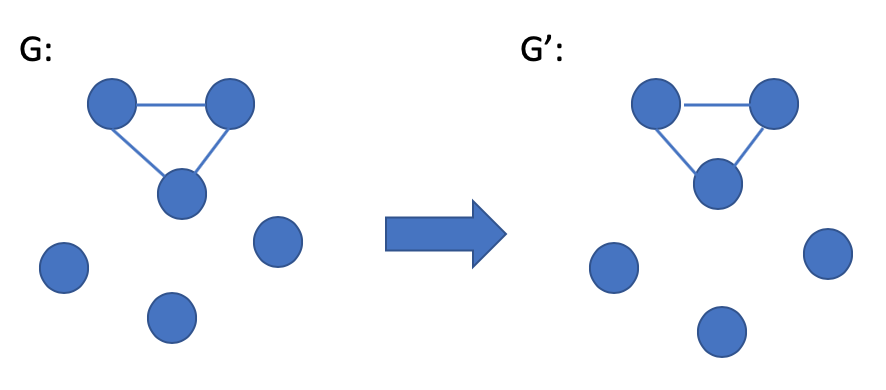
\includegraphics[scale=0.4]{images/im1.png}
  \centering
  \end{figure}
  
 In this very special case with $d=1$, the graph $G'$ after the random deletion process where we deleted vertices with probability $0$ is identical to $G$. As $G$ was not an independent set, neither is $G'$. \newline
 So, we need to do something more to $G'$ to assure we find an independent set in $G$. The easiest way to do this is to follow the algorithm proposed in 1c: for each remaining edge in $G'$, we remove the edge and one of its incident vertices.  
 
 \begin{figure}[h]
  \includegraphics[scale=0.4]{images/im2.png}
  \centering
  \end{figure}
  
  We state that the remaining vertices in $G''$ form an independent set in G. We prove this by assuming the contrary (e.g. the vertices of $G''$ are not an independent set in $G$). This means that at least two vertices $v_a$ and $v_b$ are linked by an edge in $G$. But if $v_a$ and $v_b$ are adjacent in $G$ and still both present in $G''$, this means that the edge between them was somehow deleted during the first random phase while keeping both vertices, otherwise the second phase would have removed one of them when it deleted their linking edge. This is a contradiction to how $G'$ is built, because edges only disappear if one of its incident vertices is deleted $\bot$ \newline
  Thus, we can calculate the expected number of vertices remaining in $G''$ (e.g. the expected size of the constructed independent set). So, by setting $\alpha(G)$ as the size of the independent set we constructed by this two-step process, we find: 
  \begin{equation}
      E[\alpha(G)] \geq E[C_v-C_e] = E[C_v]-E[C_e]=\frac{n}{d}-\frac{n}{2d} = \frac{n}{2d}
  \end{equation}
  It is a lower bound on the number of independent vertices, because to create $G''$, we removed a vertex for every edge so the expected number of removed vertices from $G'$ to $G''$ is at most $\frac{n}{2d}$. In the case where some vertices in $G'$ can have a bigger degree than 1, we see by looking at the example below,    that removing the centre vertex immediately leaves the rest as an independent set with more vertices than if we had removed the outer vertices (e.g. corresponding to the number of edges). So it is possible to obtain an independent set bigger than $C_v-C_e$.
   \begin{figure}[h]
  \includegraphics[scale=0.4]{images/im3.png}
  \centering
  \end{figure}
  \end{exercise}
 
  \begin{exercise}{1c} Let G be a 3-regular graph. Suppose we would like to turn our randomised experiment into an algorithm as follows. We delete every vertex of G independently with probability 2/3. Then for every edge that remain delete one of its endpoints. Derive an upper bound on the probability that this algorithm finds an independent set smaller than $(1-\epsilon)n/6$. \newline
 \emph{Answer:} Firstly, for the sake of clarity, let's give and recall the definition of some random variables that will be used in the derivation of this upper bound. 
 \begin{itemize}
 \item $\alpha(G) = \sum_{i=1}^{n} X_{v_i}$: Size of the independent vertex set returned by the two steps algorithm on the input $G=(V,E)$ with $|V| =n$ and  $|E| = \frac{nd}{2}$ (d=3 in our case).
 \item $X_{v_i}$: Indicator variable indicating if vertex $v_i \in V, i = 1,...,n$ is in the independent vertex set returned by algorithm ($X_{v_i}=1$) or if it has been deleted in the process ($X_{v_i}=0$). 
 \item $\Delta :=  n - \alpha(G)$: Number of vertices that are deleted by the algorithm.
 \end{itemize}
 In addition to that, recall the following identities and inequalities:
 \begin{itemize}
  \item \textbf{Markov's Inequality}: For any positive random variable $X$ and $\epsilon > 0$:
 \begin{equation}
 \label{eq:markov}
 P[X > \epsilon ] \leq \frac{\mathbb{E}[X]}{\epsilon}.
 \end{equation}
 \item \textbf{Chebyshev's Inequality}: For any random variable $X$ and $\epsilon > 0$:
 \begin{equation}
 \label{eq:chebychev}
 P[|X-\mathbb{E}[X]| > \epsilon ] \leq \frac{\mathrm{Var}[X]}{\epsilon^2}.
 \end{equation}
 \item For any random variable $X$:
  \begin{equation}
 \label{eq:varprop1}
\mathrm{Var}[aX + b] = a^2\mathrm{Var}[X], \quad \forall a,b \in \mathbb{R}.
 \end{equation}
 \item For any set of random variable $X_i, i = 1,...,n$:
   \begin{equation}
 \label{eq:varprop2}
\mathrm{Var}\left[\sum_{i=1}^{n} X_i\right] = \sum_{i=1}^{n}\mathrm{Var}[X_i] + \sum_{i = 1}^{n} \sum_{\substack{j=1 \\ j\neq i}}^{n}\mathrm{Cov}[X_i, X_j].
 \end{equation}
 \item For two indicator random variable $X_v$ and $X_u$:
    \begin{equation}
 \label{eq:covprop}
\mathrm{Cov}[X_u,X_v] = P[X_u=1 \cap X_v=1] -  P[X_u=1] P[X_v=1].
 \end{equation}
 \item Expectancy of the number of deleted vertices : from part 1b., we have that $\mathbb{E}[\alpha(G)] \geq \frac{n}{2d}$. So,
 \begin{equation}
 \label{eq:deltaexpectation2}
 \mathbb{E}[\Delta] = n - \mathbb{E}[\alpha(G)]\leq  n - \frac{1}{6}n = \frac{5}{6}n.
 \end{equation}
 \end{itemize}
 With this in mind, the goal of this exercise is to find an upper bound on \\ ${P[\alpha(G) < (1-\epsilon)\frac{n}{6}]}$. We can rewrite this probability as follows:

\begin{align*}
P\left[\alpha(G) < (1-\epsilon)\frac{n}{6}\right] 	& = P\left[ \alpha(G) - n < (1-\epsilon)\frac{n}{6}-n\right] & \\
							& = P\left[-\Delta < -\frac{5+\epsilon}{6}n\right]  & \\ 
							& = P\left[\Delta > \frac{5+\epsilon}{6}n\right] & \\
							& = P\left[\Delta - \mathbb{E}[\Delta] > \frac{5+\epsilon}{6}n - \mathbb{E}[\Delta] \right] & \\
							&  \overset{\eqref{eq:deltaexpectation2}}{\leq} P\left[\Delta - \mathbb{E}[\Delta] > \frac{5+\epsilon}{6}n - \frac{5}{6}n \right]	 & \\
							& = P\left[\Delta - \mathbb{E}[\Delta] > \frac{\epsilon n}{6} \right]	 & \\
							& \leq P\left[|\Delta - \mathbb{E}[\Delta]| > \frac{\epsilon n}{6} \right]	 & \\	
							& \overset{\eqref{eq:chebychev}}{\leq} \frac{36}{\epsilon^2 n^2} \mathrm{Var}[\Delta].						
\end{align*}
What we need now is an upper bound on the variance of $\Delta$. We have the following:
\begin{align*} \mathrm{Var}[\Delta]  	& =  \mathrm{Var}[n - \alpha(G)]  & \\
							& \overset{\eqref{eq:varprop1}}{=}  \mathrm{Var}[\alpha(G)]  & \\
							& = \mathrm{Var}\left[\sum_{i=1}^{n} X_{v_i}\right] & \\
							& \overset{\eqref{eq:varprop2}}{=} \sum_{i=1}^{n} \mathrm{Var}[X_{v_i}] + \sum_{i = 1}^{n} \sum_{\substack{j=1 \\ j\neq i}}^{n}\mathrm{Cov}[X_{v_i}, X_{v_j}] & \\
\end{align*} 
In order to continue, we need the distribution of the the random variables $X_{v_i}$. Since this is an indicator variable, it is a Bernoulli distribution and it has only one parameter $0 \leq p_i := P[X_{v_i}=1] \leq 1$. We have that
\begin{itemize}
\item $\mathrm{Var}[X_{v_i}] = \mathbb{E}[X_{v_i}^2]-\mathbb{E}[X_{v_i}]^2 = p_i-p_i^2 \leq 1, \quad \forall i = 1,...,n$. 
\item $\mathrm{Cov}[X_{v_i}, X_{v_j}]  \overset{\eqref{eq:covprop}}{=}P[X_{v_i}=1 \cap X_{v_j}=1] - p_ip_j = P[X_{v_i}=1 | X_{v_j}=1]p_j - p_ip_j$. To go further, we make the following observation. In expectation, for any graph $G=(V,E)$ and any vertex $v_i \in V$, knowing that another random vertex $v_j \in V$ has survived the algorithm decreases the probability that $v_i$ also survives, i.e. in average, $P[X_{v_i}=1 | X_{v_j}=1] \leq p_i$. This yields that the average of the covariance over the pairs of vertices $\{v_i, v_j\}$ is negative, and thus:
$$
 \sum_{i=1}^{n} \mathrm{Var}[X_{v_i}] + \sum_{i = 1}^{n} \sum_{\substack{j=1 \\ j\neq i}}^{n}\mathrm{Cov}[X_{v_i}, X_{v_j}] \leq \sum_{i=1}^{n} \mathrm{Var}[X_{v_i}] \leq n.
$$
\end{itemize}
Putting all these results together, we have that the following inequality:
\begin{equation}
P\left[\alpha(G) < (1-\epsilon)\frac{n}{6}\right] \leq \frac{36}{\epsilon^2 n} \overset{n\to \infty}{\to} 0.
\end{equation}
This is a good upper bound when $n$ grows but a bad one when $\epsilon$ decreases. In order to find an additional upper bound, we use Markov's inequality:
 \begin{align*}
 P\left[\alpha(G) < (1-\epsilon)\frac{n}{6}\right] 	& = P\left[\Delta > \frac{5+\epsilon}{6}n\right]  \\
 									& \overset{\eqref{eq:markov}}{\leq} \frac{6}{(5+\epsilon)n} \mathbb{E}[\Delta] \\
									& \overset{\eqref{eq:deltaexpectation2}}{\leq} \frac{6}{(5+\epsilon)n} \cdot \frac{5}{6}n \\
									& = \frac{5}{5+\epsilon} 
\end{align*}
 Finally, we can state the following:
 $$
  P\left[\alpha(G) < (1-\epsilon)\frac{n}{6}\right] \leq \min\left\{ \frac{5}{5+\epsilon}; \frac{36}{\epsilon^2 n} \right\}.
 $$
 \end{exercise}
  
  
   %%%%%%%%%% Exercise 2 %%%%%%%%%%
    \newpage
  \begin{exercise}{2a} Let $G = (V, E)$ be an undirected graph, and let $\mathcal{M} = (E, \mathcal{I})$ denote the graphic matroid of $G$. Define 
  \begin{displaymath}
  \mathcal{I}'= \{ S \subset E : E \setminus S \mbox{ contains a base of } \mathcal{I} \}.
  \end{displaymath}
Prove that $\mathcal{M}' = (E, \mathcal{I}')$ is a matroid.
 \newline
 \emph{Answer}: Recall the two properties that independent sets must satisfy for them to form a matroid $M=(E;I)$:
 \begin{align}
 & \mbox{if } X \subseteq Y \mbox{ and } Y \in \mathcal{I} \mbox{ then } X \in \mathcal{I}, \label{eq:p1}\\
 & \mbox{if } X, Y \in \mathcal{I} \mbox{ and } |Y| > |X| \mbox{ then } \exists e \in Y \setminus X : X \cup \{e\} \in \mathcal{I}. \label{eq:p2}
 \end{align}
Let's show that both of these properties are satisfied. 
\begin{enumerate}
\item Let $S \in \mathcal{I}'$ and $A \subset E$ such that $A \subseteq S$. Since $S \in \mathcal{I}'$, $E \setminus S$ contains a base of $\mathcal{I}$. Note that $(E \setminus S) \subseteq (E \setminus A)$ because $A \subseteq S$. Therefore $E \setminus A$ also contains at least one base of $\mathcal{I}$ (the same as $E \setminus S$ and maybe other ones). Hence $A \in \mathcal{I}'$.
\item Let $S,T \in \mathcal{I}$ such that $|T| > |S|$, and let $\Delta := T\setminus S \neq \emptyset$. 

First, we show that $\Delta$ is not a subset of every base $B_i \in \mathcal{I}$ that are in $E \setminus S$. Otherwise, there would be no element of $\Delta$ that can be added to $S$ so that $E\setminus S$ contains a basis of I. We do this by constructing such a case. \newline  
Let $B_T \in E \setminus T$ and $B_S \in E \setminus S$ be two bases of $\mathcal{I}$ (we know $B_T$ and $B_S$ exist because $T, S \in \mathcal{I}'$). If $\Delta \nsubseteq B_S$ then we have a delta that is not a subset of every base $B_i \in \mathcal{I}$ so $B_S \in E\setminus S \cup \Delta$. So assume $\Delta \subseteq B_S$. Recall that all the bases of a matroid have the same size. Therefore $|B_T| = |B_S|$. Now consider $B_{T\setminus S} := B_T \setminus S $. Since at most $|S\setminus T|$ elements of $B_T$ are in $S$, we have that 
\begin{equation}
 |S\setminus T| \geq |B_T| - |B_{T\setminus S}| \label{eq:lb}
\end{equation} 
Furthermore, using property \eqref{eq:p1}, we have that $B_{T\setminus S} \in \mathcal{I}$. We now distinguish two cases:
\begin{itemize}
\item $B_T \cap S = \emptyset$: In this case,  $B_T \cap S = \emptyset$ and $\Delta \nsubseteq B_T$ (in fact $\Delta \cap B_T = \emptyset$). Following the same reasoning as above for $\Delta \nsubseteq B_S$, we find an element that can be added to $S$ so that $E\setminus \cup{e}$ still has a base. 
\item $B_T \cap S \neq \emptyset$: In this case, $|B_{T\setminus S}| < |B_S|$. Defining $m = |B_S|-|B_{T\setminus S}|$, we can  construct a new base $B$ by adding $m$ new elements from $B_S$ to $B_{T\setminus S}$ using property \eqref{eq:p2} $m$ times consecutively. In other words:
\begin{equation}
B = B_{T\setminus S}  \cup \left(\bigcup_{j=1}^{m}\{e_j\}\right), \qquad e_j \in B_S \quad j = 1,..,m.
\end{equation}
 Finally, inequality \eqref{eq:lb} gives us that $m \leq |S \setminus T|$. Thus, since we've added at most $|S \setminus T|$ elements from $B_S$ and since
 \begin{displaymath}
  |B_S \cap \Delta| = |\Delta|=|T \setminus S| = |T| - |T\cap S|>  |S| - |T\cap S| = |S \setminus T|,
  \end{displaymath}
  there exists at least one edge in $\Delta$ that has not been added to $B$, i.e. $\Delta \nsubseteq B$. Again, as above, we have found a base to which $\Delta$ is not a complete subset of. 
\end{itemize}
We've therefore shown that there exists at least one base $B \in \mathcal{I}$ such that $\Delta \setminus B \neq \emptyset$.  Taking $e \in \Delta \setminus B \subseteq T\setminus S$, we have that $S \cup \{e\} \in \mathcal{I}'$ since $B \subseteq E\setminus (S \cup \{e\})$.
\end{enumerate}
 Since properties \eqref{eq:p1} and \eqref{eq:p2} hold for $\mathcal{M}'=(E,\mathcal{I}')$, it concludes the proof that $\mathcal{M}'$ is a matroid.
  \end{exercise}
  
   \begin{exercise}{2b}
  Give a polynomial time algorithm that, given an undirected graph $G = (V,E)$, determines if $G$ contains two edge disjoint spanning trees. \newline
  \emph{Answer}: Let $\mathcal{M}=(E,\mathcal{I})$ be the graphic matroid on $G$ and $\mathcal{M}'=(E,\mathcal{I}')$ the matroid defined in exercise 2a. Note that, in order to contain a spanning tree, the size of all the bases of $\mathcal{M}$ must equal $|V|-1$ (if they are bigger there is a cycle and if they are smaller then at least one vertex is not covered). Also, note that if a base $X \in \mathcal{I}$ is also in $\mathcal{I}'$, then we know, by definition of $\mathcal{I}'$, that there exists at least one base $X'$ which is edge disjoint with $X$. We can therefore state that there exists two edge disjoint spanning trees in $G$ if and only if \
 \begin{displaymath}
  \max_{X \in \mathcal{I} \cap \mathcal{I}'} |X| = |V|-1.
  \end{displaymath}
  This is clearly a matroid intersection problem as we want to find the size of the largest common independent set in $\mathcal{I}$ and $\mathcal{I}'$ and then check if its size equals $|V|-1$. The main idea of an algorithm that can solve matroid intersection problems (which is strongly inspired by \emph{Edmonds' Matroid Intersection Algorithm}) is presented below:
  \begin{enumerate}
  \item Start with a trivial set $I_0\in \mathcal{I} \cap \mathcal{I}'$.
  \item Find (if they exist) two  sets $A \in I_0$ and $B \in E \setminus I_0$ such that $|B| > |A|$ and $I_1 := (I_0\setminus A) \cup B \in \mathcal{I} \cap \mathcal{I}'$. 
  \item Repeat step 2) with $I_1$ to find $I_2$, then with $I_2$ to find $I_3$, and so on, until it is impossible to find the two sets $A$ and $B$. 
  \item Return the last set $I_n$ that could be found. 
  \end{enumerate} 
Now that we have the main idea of the algorithm, we still need to do the following in order to adapt it to our problem and to make sure it always solves it:
\begin{enumerate}
\item \textbf{\emph{Prove that, in our case, we can indeed find a trivial common independent set $I_0 \in \mathcal{I} \cap \mathcal{I}'$ (or find the solution to our problem by searching for it)}}: 
\newline
In order to find $I_0$, we can run \textsc{Greedy} on the graphic matroid $\mathcal{M} = (E,\mathcal{I})$ with edge weights $w : E \to \mathbb{R}, \, e \mapsto w(e) = 1$. Let $I$ be the set returned by \textsc{Greedy}.  By the properties of matroids, we know that $I$ is a base of $\mathcal{M}$. Several cases can appear:
\begin{itemize}
\item $|I| < |V| - 1$: In this case, we know that $G$ does not contain any spanning trees, let alone two edge disjoint spanning trees.
\item $|I| = |V| - 1$ and $E\setminus I = \emptyset$: In this case, the spanning tree is the whole set of edges $E$ and $G$ cannot contain two  edge disjoint spanning trees.
\item $|I| = |V| - 1$ and $E\setminus I \neq \emptyset$: In this case, any set $I_0 = \{e\}$ such that $e \in E\setminus I$ will satisfy $I_0 \in \mathcal{I} \cap \mathcal{I}'$. This is because a set of one edge does not contain a cycle $\Rightarrow \, I_0 \in \mathcal{I}$, and because by construction, there exist a base in $E\setminus \{e\}  \, \Rightarrow \, I_0 \in \mathcal{I}'$.
\end{itemize}
\item \textbf{\emph{Prove that the algorithm terminates}}: 
\newline
Since $|I_{k+1}| > |I_k|, \forall k = 0,...,n-1$, and since $|E| < +\infty$, this algorithm will terminate for sure ($I_n$ is at most $E$). 

\item \textbf{\emph{Prove that the algorithm returns one of the largest common independent set in $\mathcal{I}\cap\mathcal{I}'$}} :
\newline
By construction, the sets $I_k, \forall k = 0,...,n$ are common independent sets of the matroid intersection $\mathcal{M}\cap\mathcal{M}'$. Now, assume that $I_n$ the set returned by the above algorithm, i.e. there isn't any sets $A \in I_n$ and $B \in E \setminus I_n$ such that $|B| > |A|$ and $(I_n\setminus A) \cup B \in \mathcal{I} \cap \mathcal{I}'$, and assume that $I_n$ is not the largest common independent set, i.e. $I_n$ is not a base of the matroid intersection so $\exists\hat{I}\in \mathcal{I} \cap \mathcal{I}'$ such that $|I_n| < |\hat{I}|$. Let $A':= I_n \setminus \hat{I}$ and $B':= \hat{I}\setminus I_n$. It is easy to see that $A'$ and $B'$ satisfy the properties that $A$ and $B$ must satisfy, respectively:
\begin{itemize}
\item $A'=I_n \setminus \hat{I} \in I_n$,
\item $B'=\hat{I} \setminus I_n \in E\setminus I_n$,
\item $|B'| - |A'| = |\hat{I} \setminus I_n| - |I_n\setminus \hat{I}| = (|\hat{I}| - |I_n\cap \hat{I}|) - (|I_n| - |I_n\cap \hat{I}|) = |\hat{I}|-|I_n| > 0$,
\item $(I_n \setminus A')\cup B' = (I_n \setminus (I_n \setminus \hat{I}))\cup (\hat{I} \setminus I_n)= (I_n \cap \hat{I})\cup (\hat{I}\setminus I_n) = \hat{I} \in \mathcal{I}\cap\mathcal{I}'$.
\end{itemize} 
This leads to a contradiction to the fact that $I_n$ is the set returned by the algorithm (because $A$ and $B$ exists) and concludes the proof that $I_n$ is  one of the largest common independent set in $\mathcal{I}\cap\mathcal{I}'$.
\item \textbf{\emph{Design a method to find the two sets $A$ and $B$ if they exists}}: 
\newline
In order to find the sets $A$ and $B$, one can use a similar approach to the one used in the \textsc{AugmentingPath} algorithm for bipartite perfect matching problems. The goal is to create, at each iteration $k$ of the main algorithm, a directed graph $D_I^k$ whose vertices $V_{D_I^k}$ are the edges of the main graph $E$, and whose edges $E_{D_I^k} $ are separated in two sets: those that go from $E\setminus I_k $ to  $E$, and those that go from $E$ to $E\setminus I_k $. Let $E_{D_I^k}^1$ and $E_{D_I^k}^2$ be these two disjoint sets of directed edges, respectively. With this definition of $D_{I}^k$, one can already see that if we can find a path $P_k$ in $D_{I}^k$ that goes from $E\setminus I_k$ to $E\setminus I_k$, and if we let $A$ be the set of vertices of $P_k$ that are in $I_k$ and $B$ the set of vertices of $P_k$ that are in $E\setminus I_k$, we have that $A$ and $B$ satisfy the following properties:
\begin{itemize}
\item $A \in I_k$ and $B \in E\setminus I_k$,
\item $|B| > |A|$
\end{itemize}
The last thing we have to do is to make sure that $(I_k\setminus A)\cup B \in \mathcal{I}\cap\mathcal{I}'$ by carefully choosing the edges of $D_{I}^k$.  Let $E_{D_I^k}^1$ and $E_{D_I^k}^2$ be defined as follows:
\begin{align*}
E_{D_I^k}^1 & := \{(u,v) : u \in E, v \in E\setminus I, (I \setminus \{u\}) \cup \{v\} \in \mathcal{I} \},  \\
E_{D_I^k}^2 & := \{(v,u) : u \in E, v \in E\setminus I, (I \setminus \{u\}) \cup \{v\} \in \mathcal{I}' \}.
\end{align*}
Moreover, let $V_{D_I^k}^1$ and $V_{D_I^k}^2$ be defined as follows:
\begin{align*}
V_{D_I^k}^1 & := \{v \in E\setminus I : I\cup \{v\} \in \mathcal{I} \},  \\
V_{D_I^k}^2 & := \{v \in E\setminus I : I\cup \{v\} \in \mathcal{I}'\}.
\end{align*}
Lastly, let $P_k = v_0u_1v_1...u_nv_n$ be the shortest path between $V_{D_I^k}^1$ and $V_{D_I^k}^2$ in $D_{I}^k$. It can be proved that $A := I_k \cap \{u_i\}_{1\leq i \leq n}$ and $B :=  \{v_i\}_{0\leq i \leq n}$ satisfy $(I_k\setminus A)\cup B \in \mathcal{I}\cap\mathcal{I}'$. This proof is rather technical and will not be exposed here, but it can be found here:\href{https://www.mathematik.hu-berlin.de/~wilhelm/greedy-ausarbeitung.pdf}{ Lemma 13.28} \cite{Wilhelm}. In addition, the shortest path can be found in polynomial time by simply computing the shortest path from every vertices in $V_{D_I^k}^1$ to every vertices in $V_{D_I^k}^1$.
\newline
\item \emph{\textbf{Design methods to answer the queries "$I \in \mathcal{I}?$" and "$I \in \mathcal{I}'?$"}}:
\begin{itemize}
\item To answer "$I \in \mathcal{I}?$", one can simply run \textsc{DFS} on the graph $G=(V,I)$ and check for any visited vertex $v$ if there exists an adjacent vertex $u$ that has already been visited such that $v$ is not a descendent of $u$. If such a vertex $u$ is found before \textsc{DFS} terminates, then $I \not\in \mathcal{I}$. Else $I \in \mathcal{I}$. \textsc{DFS}($V,E$) runs in time $O(|E| + |V|)$ and the query can therefore be answered in time $O(|E| + |I|)$.
\item To answer "$I \in \mathcal{I}'?$", one can run \textsc{Greedy}  with edge weights $w : (E \setminus I) \to \mathbb{R}, \, e \mapsto w(e) = 1$ on the graphic matroid obtained with the graph $G=(V, E\setminus I)$ (one can use the algorithm above to answer the queries "$I \in \mathcal{I}?$" in \textsc{Greedy}). If the base returned by \textsc{Greedy} has size $|V|-1$, then $I \in \mathcal{I}'$. Else $I \not \in \mathcal{I}'$. This can be answered in time $O(|E|(|E|+|V|))$.
\end{itemize}
\end{enumerate}
Now that we have an algorithm to find a maximal common independent set $I_n \in \mathcal{I} \cap \mathcal{I}'$, we simply need to output 
\begin{itemize}
\item \emph{"$G$ contains two edge disjoint spanning trees"} if $|I_n| = |V|-1$.
\item \emph{"$G$ does not contain two edge disjoint spanning trees"} if $|I_n| < |V|-1$.
\end{itemize}
Finally, since this algorithm is a combination of loops and polynomial time elementary algorithms (no recursion), it is clear that its runtime is also polynomial.
  \end{exercise}

%\newpage
%\begin{exercise}{2b}
%Give a polynomial time algorithm that, given an undirected graph $G = (V,E)$, determines if $G$ contains two edge disjoint spanning trees (EDST). \newline
%\emph{Answer}: 
%First, in order to solve this problem in polynomial time, we need do design relatively efficient methods to answer the queries "$I \in \mathcal{I}?$" and "$I \in \mathcal{I}'?$":
%\begin{itemize}
%\item To answer "$I \in \mathcal{I}?$", one can simply run \textsc{DFS} on the graph $G=(V,I)$ and check for any visited vertex $v$ if there exists an adjacent vertex $u$ that has already been visited such that $v$ is not a descendent of $u$. If such a vertex $u$ is found before \textsc{DFS} terminates, then $I \not\in \mathcal{I}$. Else $I \in \mathcal{I}$. \textsc{DFS}($V,E$) runs in time $O(|E| + |V|)$ and the query can therefore be answered in time $O(|E| + |I|)$.
%\item To answer "$I \in \mathcal{I}'?$", one can run \textsc{Greedy}  with edge weights $w : (E \setminus I) \to \mathbb{R}, \, e \mapsto w(e) = 1$ on the graphic matroid obtained with the graph $G=(V, E\setminus I)$ (one can use the algorithm above to answer the queries "$I \in \mathcal{I}?$" in \textsc{Greedy}). If the base returned by \textsc{Greedy} has size $|V|-1$, then $I \in \mathcal{I}'$. Else $I \not \in \mathcal{I}'$. This can be answered in time $O(|E|(|E|+|V|))$.
%\end{itemize}
%With the help of these tools, we can now devise an efficient procedure to find if $G$ contains two EDST. Let $\mathcal{M}=(E,\mathcal{I})$ be the graphic matroid on $G$ and $\mathcal{M}'=(E,\mathcal{I}')$ the matroid defined in exercise 2a. Before using the main algorithm, a preliminary tests must be made on graphs $G$:  Note that in order to contain a spanning tree, the size of all the bases of $\mathcal{M}$ must equal $|V|-1$ (if more then you have a cycle, if less then at least one vertex is not covered).  This can be easily checked using \textsc{Greedy} with edge weights $w : E  \to \mathbb{R}, \, e \mapsto w(e) = 1$ on the graphic matroid $\mathcal{M}$, and then by checking the size of the base $I$ returned by the algorithm: 
%\begin{itemize}
%\item If $|I| < |V| - 1$, $G$ does not contain two EDST.
%\item If $|I| = |V| - 1$, $G$ contains at least one spanning tree and we need to run the algorithm described below to find if it has two EDST.. 
%\end{itemize}
%
%\noindent Once we know $G$ contains at least one spanning tree, we can make the following observation. Assume you can find two independent sets $I_1 \in \mathcal{I}$ and $I_2 \in \mathcal{I}'$ such that $|I_1 \cup I_2| \geq 2(|V|-1)$
%\end{exercise}
\newpage
  \begin{exercise}{3a} Show that for every $k = 1,...,n$ one has $price(e_k) \leq OPT/(n-k+1)$ \newline
  \emph{Answer.}
    Firstly, we will introduce some notation to capture the partial solutions of
    each iteration of the algorithm. In the following, by an \textit{iteration}
    of the algorithm we mean the completion of one repetition of the while loop.
    Let $m$ be the number of sets chosen by the
    greedy algorithm and $S_1, \ldots, S_m$ be the sequence of the chosen sets
    ordered by the time they were added to the solution set.
    Let $C_k = \cup_{i=1}^k S_i$ for $k = 1, \ldots, m$ and $C_0 = \emptyset$
    be the partial cover built after the $k$-th iteration of the algorithm.
    \iffalse Therefore $|C_0| =
    0$ and $|C_m| = n$. \fi Let $A_k = S_k \setminus C_{k - 1}$ for $k=  1,
    \ldots, m$ be the set of elements in
    the universe covered only after adding on the set $S_k$ to the solution.

    \iffalse
    The first observation is that $|A_i| \geq |A_j|$ for any $1 \leq i < j \leq
    m$. Following a proof by contradiction, assume that $\exists \textrm{ } i,j
    \textrm{ s.t. } 1 \leq i < j
    \leq m$ and $|A_i| < |A_j|$ then
    \begin{align*}
      |A_i| = |S_i \setminus C_{i - 1}| < |S_j \setminus C_{j - 1} | \leq |S_j \setminus C_{i - 1}|
    \end{align*}
    which contradicts the greedy step of choosing $S_i = argmax_{S \in \Fcal}| S \setminus C_{i-1}|$.
    \fi


    \begin{proof}
    Let $S^*_1, \ldots, S^*_{|OPT|} \in \Fcal$ be an optimal cover. For a fixed
    iteration $j \in \left\{1, \ldots, m\right\}$ of the algorithm, using the
    fact that $\left\{S_i^*\right\}$ is a cover, i.e. $U =
    \bigcup_i S^*_i$, the number of so far uncovered elements can be upper bounded
    as follows:
    \begin{align*}
      |U \setminus C_{j - 1}| &= \left|\left( \bigcup_i S^*_i \right) \setminus C_{j - 1}\right| \\
      &= \left| \bigcup_i (S^*_i \setminus C_{j - 1}) \right| \\
      &\leq \sum_i \left| S^*_i \setminus C_{j-1} \right| \\
      &\leq \sum_i \left| S_j \setminus C_{j-1} \right| = OPT \times |A_j|
    \end{align*}
    where the the last inequality follows from the greedy choice of $S_j$. As
    $price(e) = \frac{1}{|A_j|}$ for all $e \in A_j$ and $|U \setminus C_{j - 1}| = n -
    |C_{j - 1}|$, it follows from the above inequality that the following upper
    bound holds for the prices assigned by \textrm{Greedy}:
    \begin{align*}
      price(e) \leq \frac{OPT}{n - |C_{j - 1}|}, \forall e \in A_j\textrm{ and }j = 1, \ldots, m.
    \end{align*}
    As the elements of $A_j$ appear to the right of the elements of $C_{j-
      1}$ in the sequence $e_1, \ldots, e_n$ ordered by the time of addition, it
    follows that
    \begin{align*}
      e_k \in A_j &\Rightarrow k > |C_{j - 1}| \Rightarrow k - 1 \geq |C_{j - 1}|\\
                    &\Rightarrow price(e_k) \leq \frac{OPT}{n - |C_{j - 1}|} \leq \frac{OPT}{n  - k  +1}.
    \end{align*}
    \textit{\textbf{Remark: }}Already at this stage it is possible to foreshadow the result that will
    become apparent only at the end of the exercise. Namely, that summing through the prices of all
    the elements, we find that
    \begin{align*}
      \sum_{k = 1}^n price(e_k) \leq \sum_{k = 1}^n\frac{OPT}{ n - k  + 1} = OPT \sum_{k = 1}{n} \frac{1}{k} = H_n \times OPT.
      \end{align*}
    But the sum of all the prices of the elements is equal to the number of sets
    in the solution:
    \begin{align*}
      \sum_{i = 1}^n prices(e_i) = \sum_{j = 1}^{m} \sum_{k = 1}^{|A_j|} \frac{1}{|A_j|} = \sum_{j = 1}^m 1 = m
    \end{align*}
    Hence: $OPT_{greedy} \leq H_n OPT$.
    \end{proof}
\end{exercise}

\begin{exercise}{3b}
  The point $(y_1, \ldots, y_e) \in \R^n$ with $y_e = \frac{price(e)}{H_n}$ is a point inside the feasible
  polytope of the dual LP if and only if
  \begin{align*}
    \sum_{e \in S} y_e \leq 1 \iff \sum_{e \in S} price(e) \leq H_n, \ \forall \ S \in \Fcal
  \end{align*}
  since the $y_e \geq 0$ conditions are already trivially satisfied.
  By the construction of $price(e)$, the above sum can be written explicitly by
  summing the number of elements added at every iteration of the algorithm:
  \begin{align}
    \sum_{e \in S} price(e) = \sum_{i = 1}^m \frac{|S \cap A_i|}{|A_i|} \leq \sum_{i = 1}^m \frac{|S \cap A_i|}{|S \setminus C_{i - 1}|}
    \label{eq:3bpart1}
  \end{align}
  where the last inequality follows from the greedy step that $| S \setminus C_{i -
    1}| \leq |A_i| = |S_i \setminus C_{i - 1}|$.
  \begin{subequations}
      \label{eq:3bpart2}
  \begin{align}
\sum_{i = 1}^m \frac{|S \cap A_i|}{|S \setminus C_{i - 1}|} &= \sum_{i = 1}^m \frac{|S \setminus C_{i-1}| - |S \setminus C_{i}|}{|S \setminus C_{i - 1}|} \\
    &= \sum_{i = 1}^m \sum_{j = |S \setminus C_i| + 1}^{|S \setminus C_{i - 1}|} \frac{1}{|S \setminus C_{i - 1}|} \\
    &\leq \sum_{i = 1}^m \sum_{j = |S \setminus C_i| + 1}^{|S \setminus C_{i - 1}|} \frac{1}{j} && (|S \setminus C_{i-1}| \geq j) \\
    &= \sum_{i = 1}^m \left( H_{|S \setminus C_{i- 1}|} - H_{|S \setminus C_{i}|} \right) \\
    &= H_{|S \setminus C_{0}|} - H_{|S \setminus C_{m}|} = H_n
  \end{align}
  \end{subequations}
  Combining \autoref{eq:3bpart1} and \autoref{eq:3bpart2} yields $$\sum_{e \in S}
  price(e) \leq H_n \implies \sum_{e \in S} y_e = \sum_{e \in S} price(e)/H_n
  \leq 1$$ proving that $(y_1, \ldots, y_n)$ is a feasible solution.
\end{exercise}

\begin{exercise}{3c}
  \iffalse
  Since \scshape{Greedy} outputs a valid cover, for every element $e \in U$,
  \fi

  \begin{proof}
  Let $x_S,\, S \in \Fcal$ be the optimal cover such that $|OPT| = \sum_{S\in
    \Fcal} x_S$. Obviously, since $x_S$ is a cover, it is feasible: 
  there exists at least one $S \in \Fcal$ such that $e \in S$ and $x_S = 1$.

  In the exercise 3b we have shown that $y_e = \frac{price(e)}{H_n}$ is a
  feasible solution of the dual LP. By the Weak Duality theorem, it follows that
  \begin{align*}
    |OPT| = \sum_{S \in \Fcal} x_S \geq \sum_{e \in U} y_e = \frac{1}{H_n}\sum_{e \in U} price(e) = \frac{|OPT^{G}|}{H_n}
  \end{align*}
  Hence the greedy solution is an $H_n$-approximation of the optimal set cover problem:
  \begin{align*}
    |OPT^G| \leq H_n\times |OPT|.
  \end{align*}
  \end{proof}
\end{exercise}


 
  %%%%%%%%%% Exercise 4 %%%%%%%%%%
  \newpage
  \begin{exercise}{4a}
 Give a feasible solution to the LP relaxation of Set Cover on the instance below with value bounded by 2.
  \begin{equation}  \label{eq:instance} \begin{array}{rl}
  \mathcal{U} = \left\{ x \in \{0,1\}^d : \sum_{i=1}^dx_i=\frac{d}{2}\right\} &  \mbox{with } d \geq 2 \mbox{ an even integer}, \\
  \mathcal{F} = \{S_1, ..., S_m\} &  \mbox{with } m=d, \\
 S_i = \{x \in \mathcal{U} : x_i = 1 \} \\ c(S_i)=1 & \mbox{for } i=1,...,m.
 \end{array} 
\end{equation}
  \emph{Answer}: The LP relaxation of Set Cover is expressed as follows:
 \begin{align}
 \mbox{\textbf{Minimize:}} \quad &  \sum_{i=1}^m \alpha_i c(S_i) \label{eq:cost} \\
 \mbox{\textbf{Subject to:}} \quad & \sum_{S_i : \, x \in S_i} \alpha_i \geq 1 \qquad \forall x \in \mathcal{U} \label{eq:c1} \\
 & \alpha_i \in [0, 1] \qquad i = 1,...,m \label{eq:c2}
 \end{align}
  Observe that by construction of $\mathcal{U}$, every element $x \in \mathcal{U}$ belongs to exactly $d/2$ sets $S_i$.   Let's now prove that $\alpha^* \in \mathbb{Q}^m$ with $\alpha^*_i = 2/d, \, i=1,\ldots,m$ is a feasible solution with a cost bounded by 2.
Firstly, using the previous observation, constraint \eqref{eq:c1} is satisfied because
  \begin{equation}
  \sum_{S_i : \, x \in S_i} \alpha^*_i = \sum_{S_i : \, x \in S_i} \frac{2}{d} = \frac{d}{2}\cdot\frac{2}{d}=1, \qquad \forall x \in \mathcal{U}.
  \end{equation}
Secondly, since $m=d \geq 2$, constraint \eqref{eq:c2} is satisfied because $0 < \alpha^*_i = 2/d \leq 1, \, i = 1,...,m$.
Lastly, the cost \eqref{eq:cost} of solution $\alpha^*$ is given by
  \begin{equation}
  \label{eq:OPTLP_ub}
  \sum_{i=1}^m \alpha_i^* \underbrace{c(S_i)}_{=1} =  \sum_{i=1}^m \alpha_i^* =  \sum_{i=1}^m \frac{2}{d} = m \cdot \frac{2}{d} = d \cdot \frac{2}{d} = 2.
  \end{equation}
  This concludes the proof that $\alpha^*$ is a feasible solution with a cost not bigger than 2.
  \end{exercise}
  \begin{exercise}{4b}
  Prove that at least $d/2 + 1$ sets are needed to cover the universe $\mathcal{U}$. \newline
  \emph{Answer}: 
  \begin{itemize}
  \item Firstly, let's show that for any collection of sets $\mathcal{G}$ with size $|\mathcal{G}| \leq \frac{d}{2} $, there exists at least one element $\hat{x} \in \mathcal{U}$ that is not covered by $\mathcal{G}$:
  \newline 
  
  Let $I = \{ i : S_i \notin \mathcal{G}\}$. If $|\mathcal{G}| \leq \frac{d}{2}$, then $|I| \geq \frac{d}{2}$ and there exists at least one set $I' \subseteq I$ with size $|I'| = \frac{d}{2}$. Moreover, let $\hat{x} \in \{0,1\}^d$ be defined as follows:
  \begin{displaymath}
  \hat{x}_i = \left\{ \begin{array}{rcl}1 & \mbox{if} & i \in I', \\ 0 & \mbox{if} & i \in \{1,..,d\}\setminus I'. \end{array}\right.
  \end{displaymath}
  Observe that since $|I'|=\frac{d}{2}$, $\hat{x} \in \mathcal{U}$. Finally, by construction of $\hat{x}$ (as it indicates sets that were not chosen), we have that $\hat{x} \notin S_i, \, \forall S_i \in \mathcal{G}$. This concludes the proof that the universe $\mathcal{U}$ cannot be covered with a collection of set $\mathcal{G}$ with size strictly lower than $\frac{d}{2} + 1$. 
  
 \item Secondly, let's show that a collection of sets $\mathcal{G}$ with size $|\mathcal{G}| \geq \frac{d}{2} + 1$ covers every element $x \in \mathcal{U}$:
 \newline 
 
 As noted previously, every element $x \in \mathcal{U}$ belongs to exactly $\frac{d}{2}$ sets $S_i$. At least one of these sets must belong to any collection of sets $\mathcal{G}$ with size $|\mathcal{G}| \geq \frac{d}{2} + 1$ (because at most $\frac{d}{2}-1$ sets don't belong to such a $\mathcal{G}$). This concludes the proof.
 \end{itemize}
  \end{exercise}
  
  \begin{exercise}{4c}
  Conclude that the integrality gap of the LP relaxation of Set Cover on a universe $\mathcal{U}$ of size $n$ is $\Omega(\log n)$. \newline
  \emph{Answer}: Let $\mathcal{I}$ be the set of all instances of a Set Cover problem with universe of size $n$. The integrality gap $g$ of the LP relaxation of Set Cover is defined as follows:
  \begin{displaymath}
  g = \max_{I\in \mathcal{I}} \frac{ OPT(I)}{OPT_{LP}(I)},
  \end{displaymath}
  where $OPT(I)$ and $OPT_{LP}(I)$ are optimal solutions for the instance $I$ of Set Cover and its LP relaxation, respectively. Let $\hat{I}$ denote the instance of the Set Cover problem discussed in this exercise and defined by \eqref{eq:instance}. We found that $OPT_{LP}(\hat{I}) \leq 2$ (Eq. \eqref{eq:OPTLP_ub}) and that $OPT(\hat{I}) \geq \frac{d}{2} + 1$ since any collection of set covering the universe $\mathcal{U}$ must contain at least $\frac{d}{2} + 1$ sets. This yields
  \begin{equation}
  \label{eq:intgap}
    g = \max_{I\in \mathcal{I}} \frac{ OPT(I)}{OPT_{LP}(I)} \geq \frac{ OPT(\hat{I})}{OPT_{LP}(\hat{I})} \geq \frac{\frac{d}{2}+1}{2} \geq \frac{d}{4}.
  \end{equation}
  Finally, note that the size $n$ of the universe $\mathcal{U}$  is exactly the number of ways you can choose $\frac{d}{2}$ elements among $d$, i.e. $n =\binom{d}{d/2}$. However, since $\mathcal{U}$ is a subset of $\{0,1\}^d$, its size $n$ is smaller than $2^d$. In other words, $\log(n) \leq d$. Using this and Eq. \eqref{eq:intgap}, we have that
  \begin{displaymath}
  g \geq \frac{d}{4} \geq \frac{\log(n)}{4} \quad \Rightarrow \quad g \in \Omega(\log(n)).
  \end{displaymath}
  This concludes the proof.
  
  \end{exercise}


 
 
  \begin{exercise}{5}
    \definecolor{blue-violet}{rgb}{0.66, 0.0, 0.66}
    The code of the implementation is attached in the appendix. The successful
    submission on the Codeforces Online Judge is: 

    \url{https://codeforces.com/group/TUksowRwAk/contest/272033/submission/73203204}
    by the contestant \href{https://codeforces.com/profile/PineMarten}{\textbf{\color{blue-violet}PineMarten}}.
  \end{exercise}

  \section*{Appendix}
  \subsection*{C++ Code}
  \lstinputlisting[language=C++]{exercise5.cpp}

\newpage  
 \begin{thebibliography}{9}
\bibitem{Wilhelm} 
T.Summary, P.Wilhelm: Greedy Algorithm And
Matroid Intersection Algorithm,
\\\texttt{https://www.mathematik.hu-berlin.de/\~{}wilhelm/greedy-ausarbeitung.pdf}
\end{thebibliography}
 
\end{document}

